\chapter{Literature Review}
The real-world localization and mapping problem addresses a key problem in robot navigation. It is complicated and hard. Nothing is perfect in real world. Sensors are noisy and have limited capabilities. Actuators may result in unexpected results. These conditions pushed robotic researchers to find probabilistic solutions \cite{thrun2005}. In this chapter, I will cover the terminology, types and most widely used methods for the localization and mapping problem. Most of the probabilistic solutions are subsets of state estimation techniques. To understand the methods better, I will start with the definition of the state estimation problem and its specific implementations. Then, the problem definition and the most common methods will be given.

\section{State Estimation Problem}
State estimation problem, also known as recursive Bayesian estimation, is a general problem which addresses recursively estimating an observable random variable given control inputs and perceptions. The system is often modelled as a Hidden Markov Model where the random variable is the state, observations are the perceptions of the agent and the belief state is a probability distribution on the state space. At time t, I will denote the state as \text{ $x_{t}$}, the perception as \text{ $z_{t}$}, the control input as \text{ $u_{t}$}, and the belief state as \text{ $bel(x_{t})$}. The evolution of the system and the filter is shown in Figure 2.1. The recursive filter means that, a belief at time t is calculated from the belief at time \text{$t-1$}.

The actual difficulty in estimating a random variable is representing the belief state. Since the space is continuous, representing the actual belief state is impossible in practice. There are different state estimation algorithms which overcome this difficulty for different sets of assumptions.


\begin{figure}[!htbp]
\centering
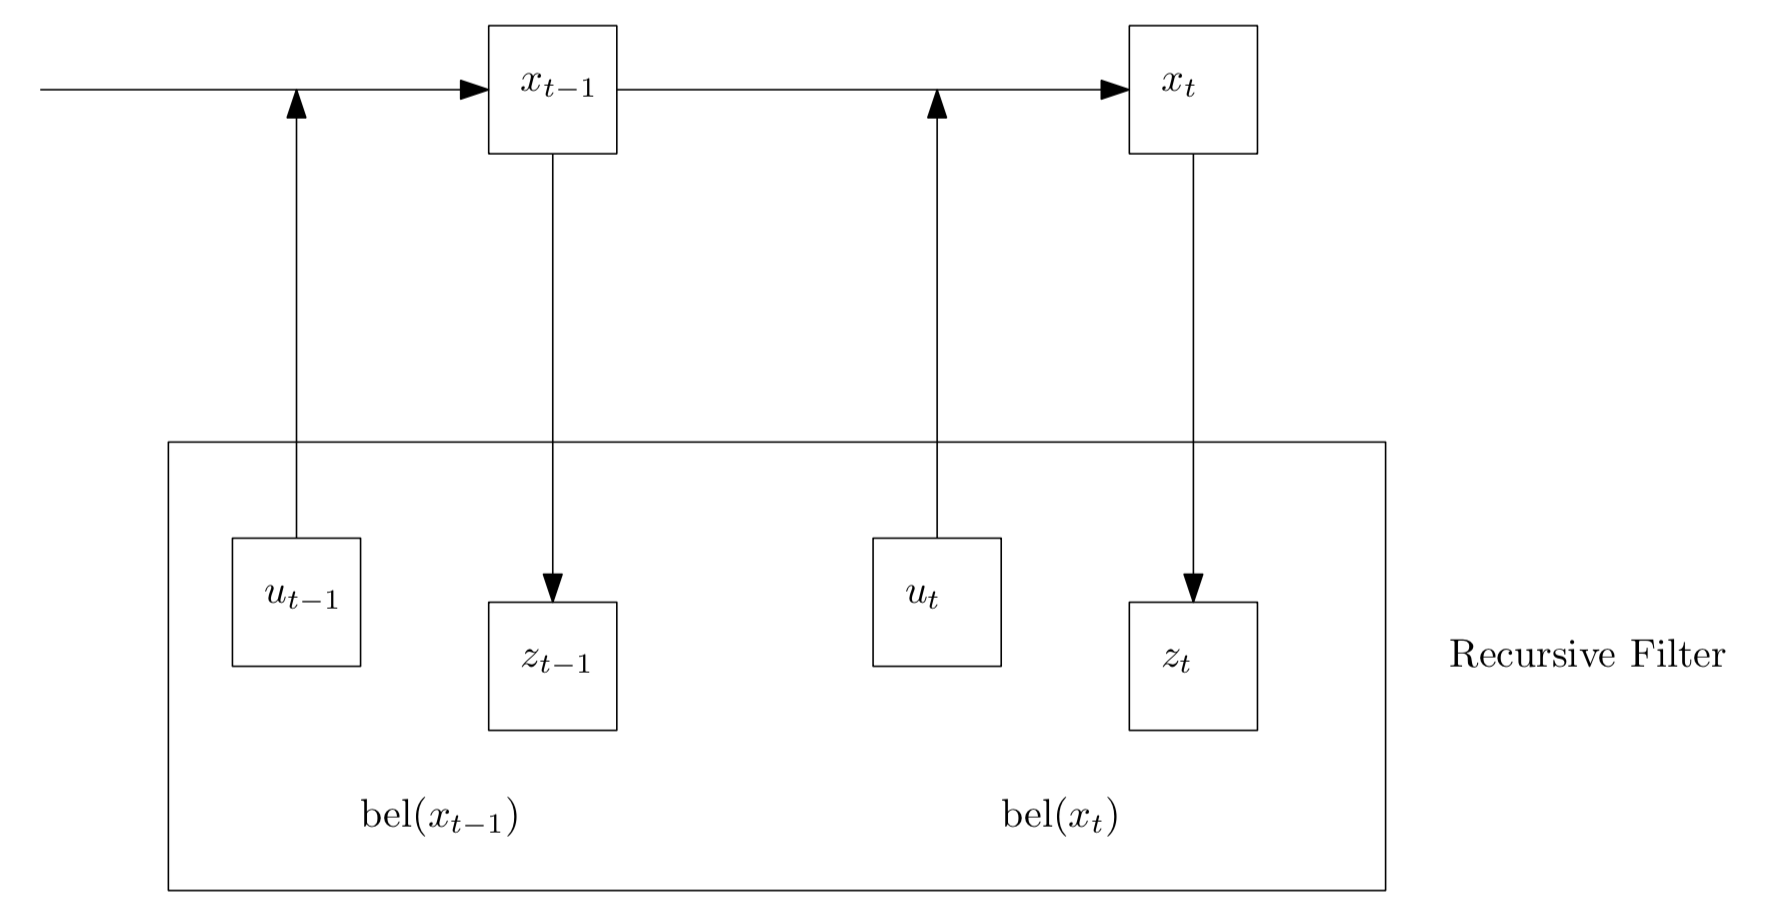
\includegraphics[width=\textwidth]{thesisChapters/images/figure21.png}
\caption{Recursive State Estimation}
\end{figure}



\subsection{Bayes Filter}
The most general algorithm for calculating the belief state is the Bayesian Filter. Each recursive state is completed in two steps. First the belief \text{ $bel(x_{t})$} is predicted using the control \text{ $u_{t}$ } and the previous belief \text{$bel(x_{t-1})$} . In the second step, the predicted belief is corrected with the perception \text{ $z_{t}$} \cite{thrun2005}. The pseudo-algorithm for the Bayes Filter is given in Figure 2.2.

The first step in the algorithm is called the prediction step, where the belief state is predicted with the control input and the uncertainty increases. Subsequently, the second step is the update step, where the predicted belief state is corrected with the observations and the uncertainty decreases. 

\begin{figure}[!htbp]
\centering
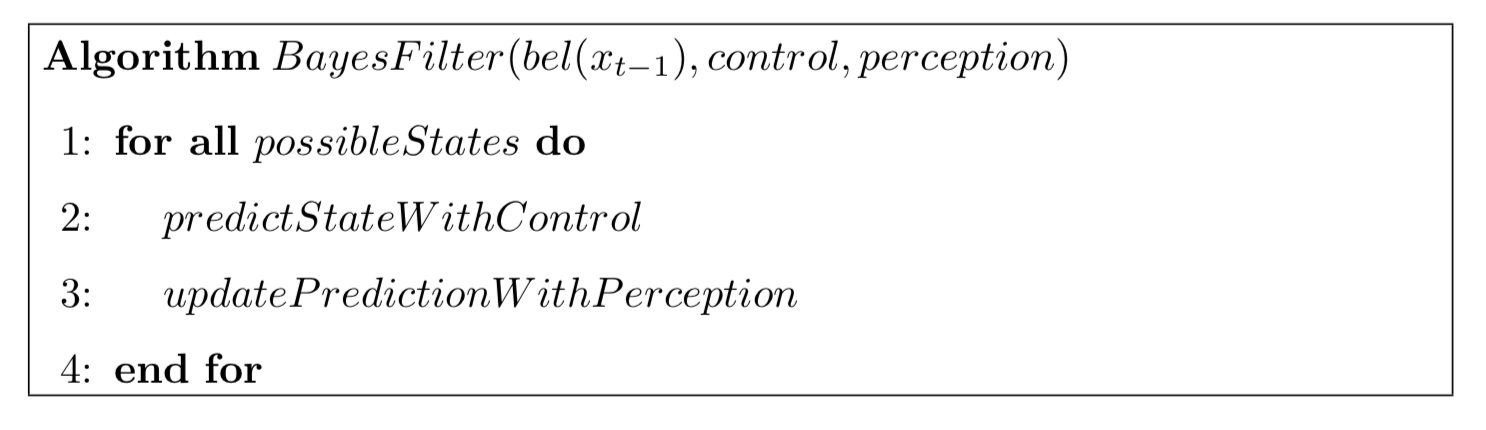
\includegraphics[width=\textwidth]{thesisChapters/images/figure22.png}
\caption{The pseudo-algorithm for Bayes Filter}
\end{figure}

Another important feature of the Bayes Filter is that at time t, the belief state only depends on the previous belief state, control input and observations. The formal algorithm is given in Figure 2.3.

\begin{figure}[!htbp]
\centering
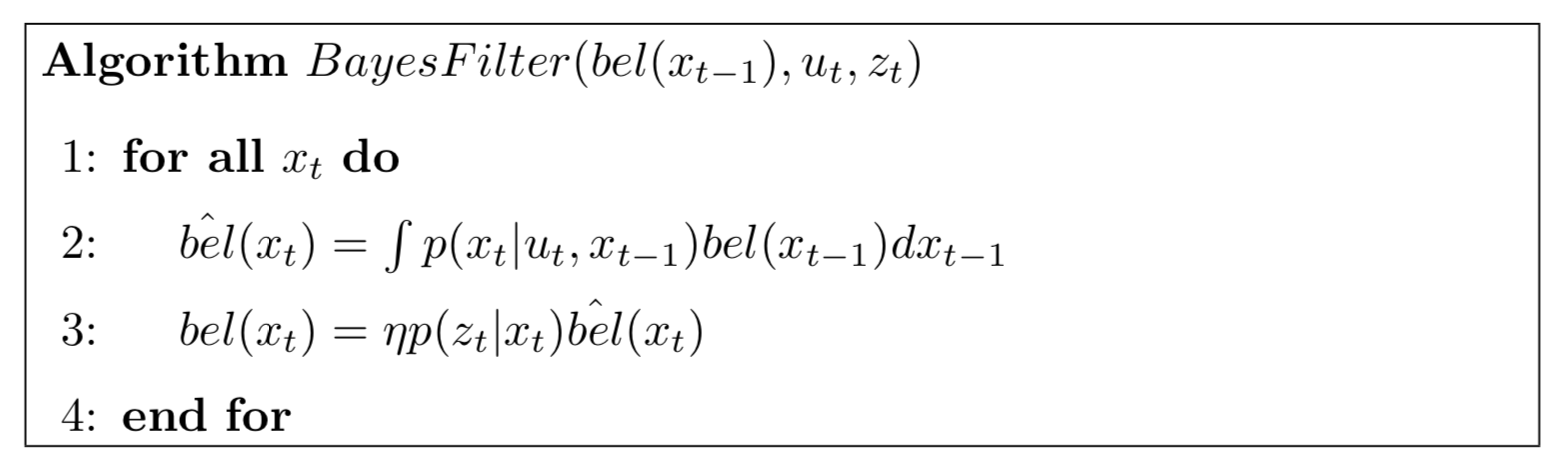
\includegraphics[width=\textwidth]{thesisChapters/images/figure23.png}
\caption{The Bayes Filter algorithm with equations}
\end{figure}


The \text{ $bel(x_{t})$} is the predicted, but uncorrected belief state. The corrected state estimation is represented as \text{ $bel(x_{t})$}. In the rest of the Thesis, “hat” symbol indicates the predicted value of a variable. The distribution p(xt|ut,xt−1) specifies the control model where \text{ $u_{t}$} represents the control input and p(zt|xt) specifies the observation model where \text{ $z_{t}$} represents the observation. To apply any kind of Bayes filter to a problem, these distributions should be specified.

The Bayes Filter is defined in continuous state spaces and most of the implementations are special cases of the Bayes Filter with different assumptions.

\section{Mobile Robot Localization Problem}
The localization problem is the problem of estimating the position of a robot given the map of the environment, observations and odometry readings. Before proceeding with the types of localization problem and solution methods, the elements should be explained.

\subsection{RobotPose}
The state to be estimated in the localization problem is the position of the robot in the 2-dimensional environment at time \text{t}.

$p_{t} = \{p_{x,t},p_{y,t},p_{\theta,t}\}$

where \text{$p_{x}$} and \text{$p_{y}$} are cartesian coordinates of the robot and \text{$p_{\theta}$} is the orientation of the robot.

In some domains, 3-dimensional position may be estimated where state vector has six elements (three for position, three for orientation). However, it is beyond the scope of this work.

\subsection{Maps}
In the localization problem, the robot is given a map of the environment in the beginning. A map contains the exact locations of all relevant entities in a finite environment. There are two types of map of the environment.

\begin{itemize}
  \item \textbf{Location Based Maps}
  In location based maps, each map entry in the map holds a property for a location in the map.
  \item \textbf{Feature Based Maps}
  In feature based maps, each map entry in the map holds the location and properties for an object in the map. The feature based maps generate two kinds of problem;
  \begin{itemize}
    \item The Known Correspondence Problem, where a robot can match the perceptions with the entities in the map,
    \item The Unknown Correspondence Problem, where a robot cannot match the perceptions with the entities in the map.
  \end{itemize}
\end{itemize}

For the feature based maps, I will denote a map as M. The map represents all the known landmarks.

$M = m_{1}, m_{2}, ..., m_{L}$ where 
$m_{i} = \ p_x^i\ , \ p_y^i\ $

Each entity \text{$m_{i}$} in the map represents the cartesian coordinate of the corresponding landmark in the global coordinate frame.

\subsection{Observations}
The robot has several sensors and can observe the entities from the map it is given. The observation format may vary with sensor type or observation algorithm type, generally the representation of a set of observations is, :

\text{$Z_{t} = \{  z_t^1 , z_t^2,..., z_t^K \} $} where

\text{$  z_t^i $} can be the bearing $ \theta_{i}$ and the distance  \text{$l_{i}$}, or both distance and bearing  \text{$l_{i}$}, 
$ \theta_{i}$  of the landmark to the robot.



The observation may come from different sensor types and the observation model \text{$ p( z_t^i|x_{t} ) $} of each type is given to the robot. For instance, if the observation comes from a laser scan as distance readings, and the map is given as a location based map (occupancy grid map), then, a likelihood field is formed and observation model is calculated accordingly as in Figure 2.4.

\begin{figure}[!htbp]
\centering
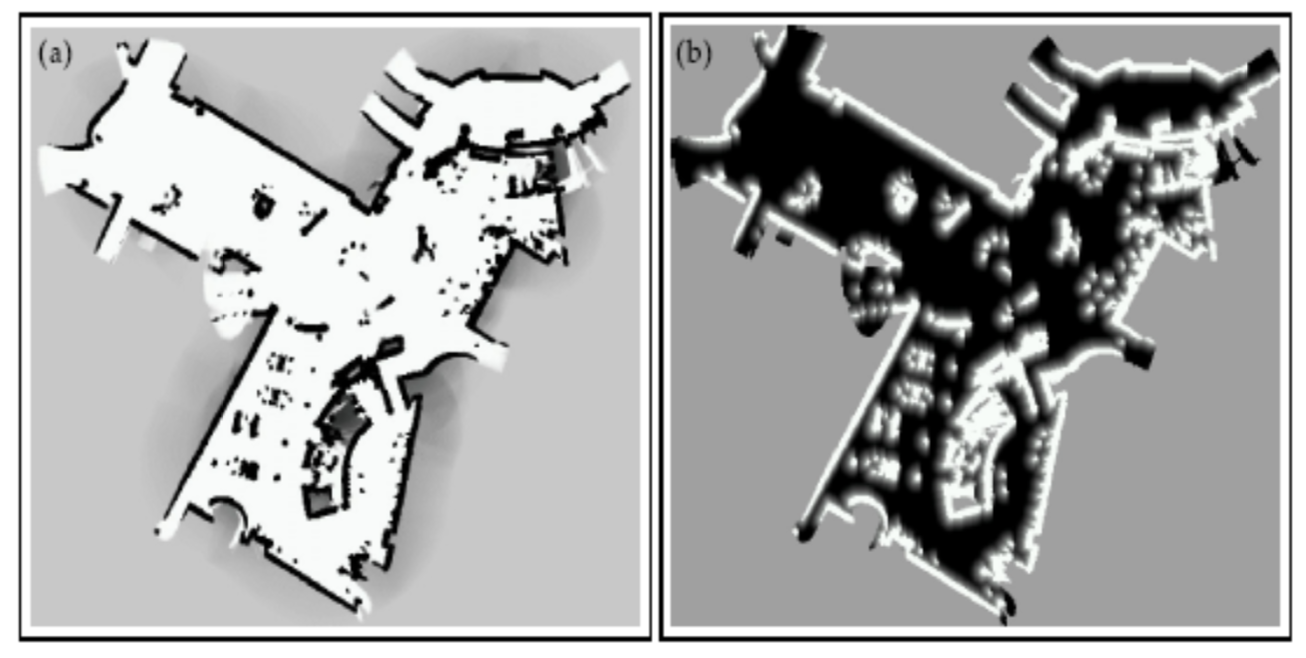
\includegraphics[width=\textwidth]{thesisChapters/images/figure24.png}
\caption{Observation model for a laser sensor. On the left, occupancy grid map. On the right, pre-calculated likelihood field. White regions represents observations with high probability \cite{thrun2005}}
\end{figure}

If the observation comes from a feature based map, the observation model is generally selected Gaussian.

\subsection{Odometry}
The odometry readings in a robot are control inputs for the localization problem. At each time step, it is assumed that robot can tell how far it has travelled with directions. The odometry readings are often represented as

$u_{t} = \{ \Delta x, \Delta y, \Delta \theta \}$

where \text{$\Delta x$} is the forward displacement, \text{$\Delta y$} is sideways displacement and \text{$\Delta \theta$} is the change in orientation. The uncertainty is modelled as Gaussian distribution. In Figure 2.5, a sample displacement reading is given.

\begin{figure}[!htbp]
\centering
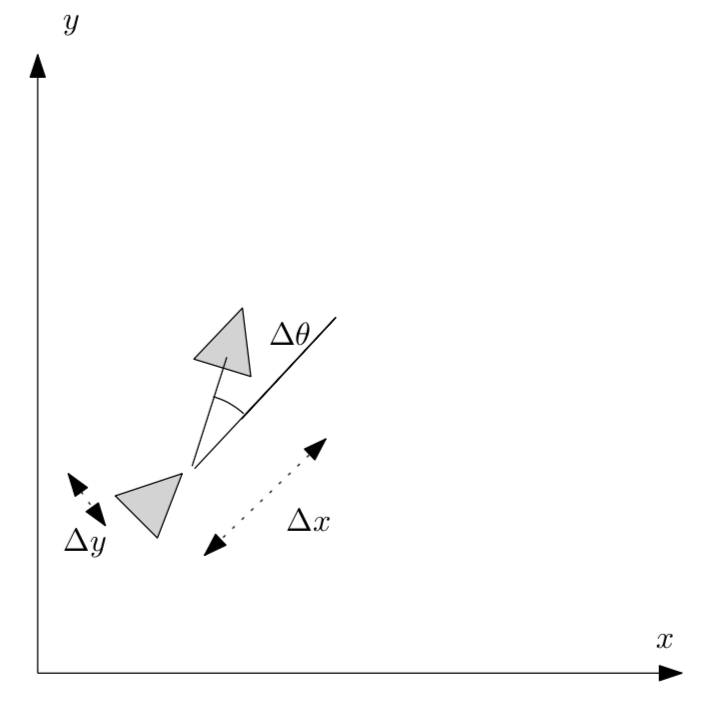
\includegraphics[width=8cm,height=8cm,angle=0]{thesisChapters/images/figure25.png}
\caption{Odometry readings of a robot}
\end{figure}

The control model function of a robot is
$x_{t+1} = g(u_{t},x_{t})$
and the element-wise definition is

\[
\begin{bmatrix}
    p_{x,t+1}       & \\
    p_{y,t+1}       & \\
    p_{\theta,t+1} 
\end{bmatrix}
=
\begin{bmatrix}
    p_{x,t} + d_{x,t}cos(p_{\theta,t}) - d_{y,t}sin(p_{\theta,t}) & \\
    p_{y,t} + d_{x,t}sin(p_{\theta,t}) - d_{y,t}cos(p_{\theta,t}) & \\
    \Delta \theta_{t} + p_{\theta,t} 
\end{bmatrix}
\]

Since the uncertainty model is Gaussian

$p(x_{t+1}|u_{t}, x_{t}) = N(x_{t+1};g(u_{t}, x_{t}), Q_{t})$

where where $Q_{t}$ is the uncertainty covariance. The probability of a state given the previous state and the odometry can be calculated as

\[ p(x_{t+1}|u_{t}, x_{t}) = \frac{1}{(2\pi)(|Q_{t}|)ˆ0.5}  *  -0.5(x_{t+1} - g(u_{t}, x_{t}) Q_{t}( x_{t+1} - g(u_{t}, x_{t}) ))\]

\section{Simultaneous Localization And Mapping}
Simultaneous localization and mapping is a problem where a moving object needs to build a map of an unknown environment, while simultaneously calculating its position within this map. \cite{gamini2001}
There are several areas which could benefit from having autonomous vehicles with SLAM algorithms implemented. Examples would be the mining industry, underwater exploration, and planetary exploration.\cite{gamini2001} The SLAM problem in general can be formulated using a probability density function denoted $p(x_{t} , m|z_{1:t} , u_{1:t} )$, where $x_{t}$ is the position of the vehicle, m is the map, and $z_{1:t}$ is a vector of all measurements. $u_{1:t}$ is a vector of the control signals of the vehicle, which is either the control commands themselves or odometry, depending on the application.

\subsection{Data Association}
Basically, the concept data association is to investigate the relationship between older data and new data gathered. In a SLAM context it is of necessity to relate older measurements to newer measurements. This enables the process of determining the locations of landmarks in the environment, and thus this also gives information regarding the robots position within the map. \cite{mit2017}

\subsection{Loop closure}
The concept of loop closure in a SLAM context is the ability of a vehicle to recognize that a location has already been visited. By applying a loop closure algorithm, the accuracy of both the map and the vehicles position within the map can be increased. \cite{yifan2016} However, this is not an easy task to perform, due to the fact that the operating environment of the vehicle could contain similar structural circumstances as previously visited locations. In that case if the loop closure algorithm performs poorly, it could lead to a faulty loop closure, which could corrupt both the map as well as the pose of the vehicle within the map. \cite{yifan2016}

\subsection{Full SLAM and online SLAM}
There are two different types of SLAM problems. The online SLAM problem of which only the current pose $x_{t}$ and the map m are expressed, given the control input $u_{1:t}$ and measurements $z_{1:t}$. As well as the full SLAM problem which expresses the entire trajectory of the robot. The PDF of the full SLAM problem is denoted as $p(x_{t} , m|z_{1:t} , u_{1:t} )$, where all the poses of the robot are considered, including its initial pose $x_{0}$. \cite{curotto2016}

\subsection{General Models for SLAM Problem}
A motion model for the SLAM problem can be described by
$x_{t} =g(u_{t},x_{t−1})+ \delta_{t}$
where the current pose $x_{t}$ depends on the possible nonlinear function $g(u_{t}, x_{t−1})$, with $u_{t}$ being the control input, $x_{t-1}$ the previous pose and δt being a random Gaussian variable with zero mean.\cite{curotto2016}

A measurement model for the SLAM problem can be described by
$z_{t}=h(x_{t},m)+\epsilon_{t}$
where the current measurement $z_{t}$, depends on the possible nonlinear function $h(x_{t},m)$, where $x_{t}$ denotes the current pose, m represents the map, $\epsilon_{t}$ a random Gaussian variable with zero mean.\cite{curotto2016}

\subsection{EKF SLAM Algorithm}
The EKF SLAM (Extended Kalman Filter) approach of solving the SLAM problem is by using sensor data gathered from the movement and rotation of the robot. This can be done by for example using wheel encoders and a gyroscope. Furthermore, it is also necessary to gather information of the environment by, for example, using a Laser Range Finder (LIDAR). With this data, the algorithm keeps track of where the robot is likely positioned within a map, as well as keeping track of specific landmarks observed.\cite{mit2017}

When the robot is turned on, the sensors on the robot such as the wheel encoders and the gyroscope will gather information of the positioning of the robot. Moreover, landmarks from the environment are also extracted based on new observations from the LIDAR which is mounted on the robot. These new observations are associated with previous observations and updated in the EKF algorithm. However, if an observation of a landmark cannot be associated to a previous observation the observation itself is presented to the EKF algorithm as a new observation.\cite{mit2017} This process is illustrated in Fig. 2.6.

\begin{figure}[!htbp]
\centering
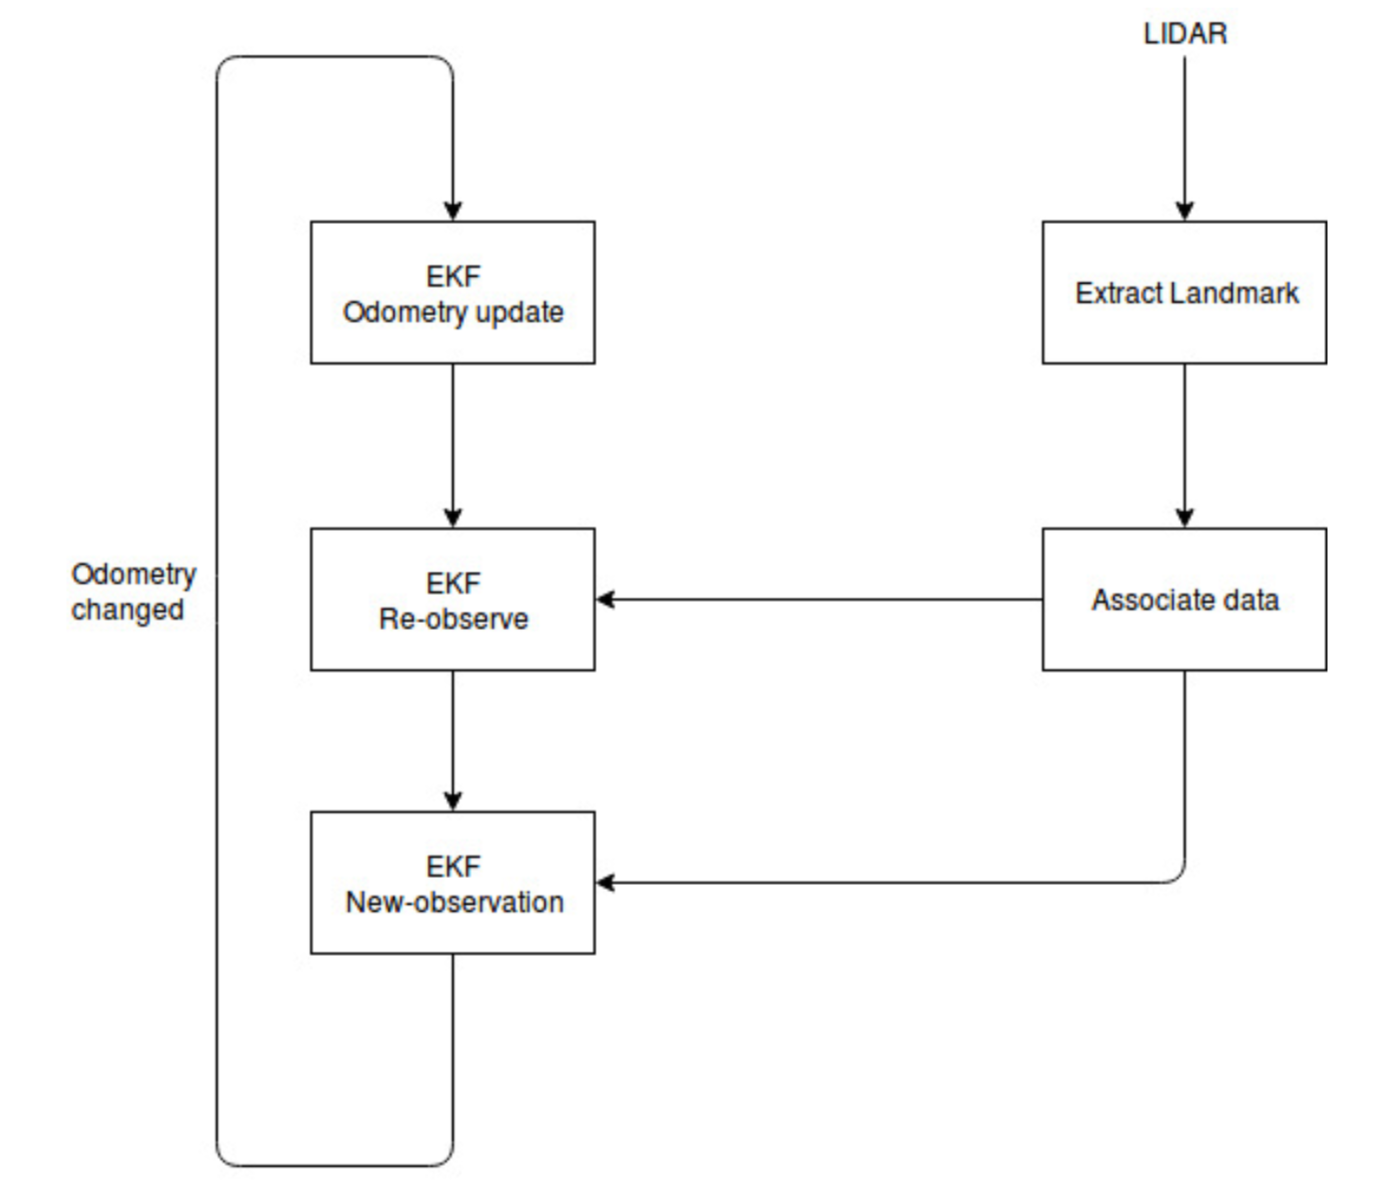
\includegraphics[width=10cm,height=10cm,angle=0]{thesisChapters/images/figure26.png}
\caption{EKF SLAM algorithm \cite{yifan2016}}
\end{figure}

First and foremost, the robot localizes itself within the map being created using observed landmarks and information from the sensors. The landmarks should preferably be observable from multiple angles, as well as not being separated from other landmarks. These prerequisites gives the EKF algorithm a good possibility to distinguish between landmarks at a later time. Moreover, the land- marks being used should also be stationary. \cite{yifan2016}


To describe the EKF SLAM process in short terms, it consists of two stages:

\begin{itemize}
  \item \textbf{Prediction step}
    \begin{itemize}
        \item \textbf{}
        Predict the current state expressed by the predicted mean and the predicted covariance. These are being calculated based on control input, matrices, the previous covariance and the previous mean. \cite{cyrill2012}
    \end{itemize}
  \item \textbf{Correction step}
    \begin{itemize}
        \item \textbf{}
        First and foremost, the idea behind the correction step is the data association. The main idea behind associating data in a SLAM context is to distinguish between an earlier observed landmark and a newly ob- served one. \cite{cyrill2012} When a new measurement has occurred the procedure is as following:
        
        \begin{itemize}
            \item Store the locations of newly observed landmarks.\cite{cyrill2012}
            \item Associate previously observed landmarks with newly observe dones. \cite{cyrill2012}
        \end{itemize}
        
        Furthermore, the correction gain, also known as the Kalman gain is computed. Basically, it is a correction gain factor necessary to up- date the current mean and covariance of the current state. The cur- rent mean and covariance is not only dependent on the Kalman gain though, but they are also taking the predicted mean and the predicted covariance and the measurement into account. \cite{cyrill2012}
    \end{itemize}
  
\end{itemize}

\subsection{EKF SLAM Algorithm Computational Complexity}
The computational cost of the EKF SLAM algorithm is quite costly in comparison to other SLAM algorithms. When new landmarks are detected, they are added to the state vector of the filter, and the map of with N identified landmarks, will increase linearily. \cite{samsuri2015} In terms of numbers, the use of memory is \text{O(\[ N^{2}\])} . The computation cost of computing one step of the algorithm is approximately \text{O(\[ N^{2}\])} \cite{cyrill2012} \cite{bozao2010}, the complete cost for computing the whole algorithm is \text{O(\[ N^{3}\])}, heavily dependant on the size of the map \cite{bozao2010}.


\subsection{Evaluation of SLAM}
There are several parameters of interest when discussing SLAM algorithms, some of which have been investigated are the following: robustness, efficiency and ROS compatibility. These parameters are evaluated and compared to each other below.

\begin{itemize}
    \item \textbf{EKF}
        \begin{itemize}
            \item Robustness
                A faulty data association will result in erroneous future results, thus the robustness of the EKF algorithm is low. \cite{thrun2005}
            \item Efficiency
                The total computational cost of executing the algorithm is O(N3), to a great degree dependant on the size of the map \cite{bozao2010}. In conclusion this makes the EKF SLAM algorithm more suitable for smaller maps containing fewer landmarks due to the heavy computational load.\cite{cyrill2012} However, as stated in 3.2.3 the localization and data association part can be difficult when the landmarks in the environment are few. \cite{thrun2005}
            \item ROS Compatibility
                Implemented in the mrpt\_ekf\_slam\_2d package.
        \end{itemize}    
    \item \textbf{FastSLAM}
        \begin{itemize}
            \item Robustness
                The Fast SLAM algorithm is significantly more robust than the EKF SLAM algorithm due to the fact that the data association from measurements to landmarks is particle-based which reduces the impact of a wrong data association.
            \item Efficiency
                The total computational cost is stated as \text{O(\[ MLog(N)\])}, meaning that the complexity is due to the number of particles M and the number of landmarks N. \cite{michael2007}
            \item ROS Compatibility
                Implemented in the gMapping package.
        \end{itemize}  
    \item \textbf{GraphSLAM}
        \begin{itemize}
            \item Robustness
                The robustness of the Graph-SLAM algorithm is higher than the EKF algorithm, partly due to the fact that older data associations can be reexamined if a wrong data association has been performed. Basically, this reduces the risk of producing erroneous future data associations thus increasing the robustness.
            \item Efficiency
                The use of memory is linearly dependent in comparison to the EKF algorithm which uses \text{O(\[ N^{2}\])} based on number of landmarks N Moreover, the computational load is time dependent, thus if the path is long the algorithm can be quite costly. \cite{thrun2005}
            \item ROS Compatibility
                Implemented in the slam\_karto package.
        \end{itemize}  
\end{itemize}

From what can be read above, the EKF SLAM algorithm is not too robust, while both the GraphSLAM algorithm and the FastSLAM algorithm have a higher robustness. Moreover, in terms of efficiency the EKF SLAM algorithm is very costly. Given that all algorithms have been implemented in ROS packages, each of these are viable choices. However, as the EKF SLAM algorithm lacks in both robustness and effeciency, the conclusion of using other more effective algorithms such as the FastSLAM or GraphSLAM instead of the EKF algorithm can be reached. These algorithms are able to efficiently deal with maps containing more land- marks, as well as larger maps in terms of sheer size. With maps containing a cou- ple of hundred landmarks, for example when trying to map the outside world, the computational complexity of the EKF algorithm could prove to be a huge problem to deal with. \cite{thrun2013}, \cite{thrun2005}